\documentclass[../thesis.tex]{subfiles}
%\addbibresource{../library.bib}
\begin{document}
\chapter{Transient and Steady-State Dynamics}\label{sec:unified}

This section is an extension of my previous work entitled ``\textit{Unified analysis of transient and steady-state electrophosphorescence using exciton and polaron dynamics modeling}''.\supercite{Hershey2016}

\section{Motivation}

\begin{wrapfigure}{R}{0.5\textwidth}
\centering
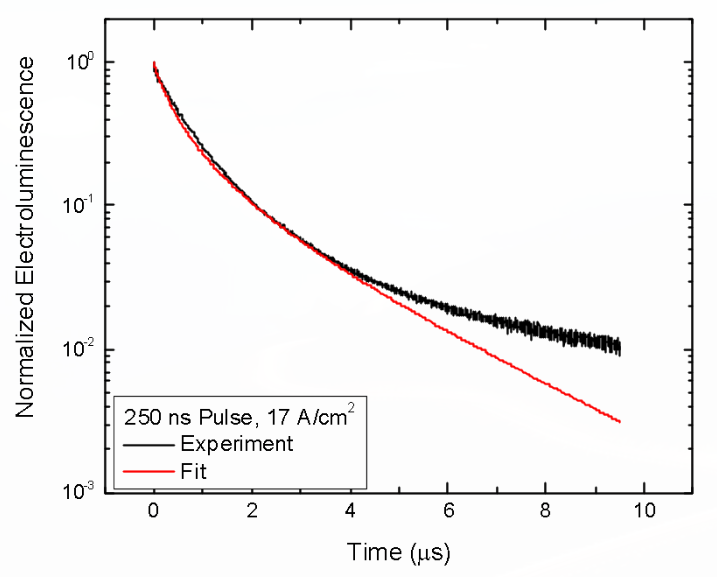
\includegraphics[width=0.48\textwidth]{unified/bad_fit}
\caption{Fitting the transient electroluminescence decay without polaron dynamics.}
\label{fig:bad_fit}
\end{wrapfigure}

As discussed in Chapter \ref{sec:oleds}, modern OLEDs are typically based around Phosphorescent emitters in order to realize 100\% internal efficiencies.\supercite{Baldo2000,Baldo1998a,Tsutsui1999,OBrien1999a}
However, these phosphorescent emitters, while allowing emission out of the triplet excitonic state, also suffer from the drawback of a longer exciton lifetime, typically on the order of 10$^{-6}$-10$^{-3}$ s.\supercite{Baldo1998a,Holmes2003}
An increased lifetime leads to a larger steady-state triplet exciton density compared to a fluorescent device operating at the same luminance.  
This becomes problematic at the high current densities associated with high brightness due to well documented quenching events.\supercite{Reineke2007,Reineke2007a,Reineke2009,Mezyk2005,Kalinowski2002,Song2010,Erickson2014}
These quenching events lead to a reduced quantum efficiency at high-current, and termed the ``Efficiency roll-off''.  


Efficiency roll-off is well attributed to quenching and is ubiquitous to phosphorescent OLED behavior.\supercite{Reineke2007,Erickson2014,Murawski2013,Giebink2008c}
While previous works have attributed the roll-off to quenching, they have failed to provide a complete picture of the exciton and charge dynamics within the device.
All of these works have utilized a differential equations model for the exciton dynamics, solved in the steady state.
This becomes apparent when investigating the transient electroluminescnce (EL), where a transient voltage pulse, on the order of 500 ns is applied to the device and the resulting luminance is recorded as a function of time.  
Figure \ref{fig:bad_fit} is an attempt to fit the transient luminance decay using the model presented by Reineke \textit{et al.}\supercite{Reineke2007} which well fits the efficiency roll-off.  
Indeed, this is a well known problem with existing models, and previous attempts to model the transient EL have utilized an empirical biexponential function to quantifiy the decay.\supercite{Erickson2014,Giebink2008c,Baldo2000a,Zhang2012}
In addition to failing to replicate the luminance decay, no known previous efforts have been made in trying to replicate the experimental transient EL luminance rise.

\begin{wrapfigure}{R}{0.5\textwidth}
\centering
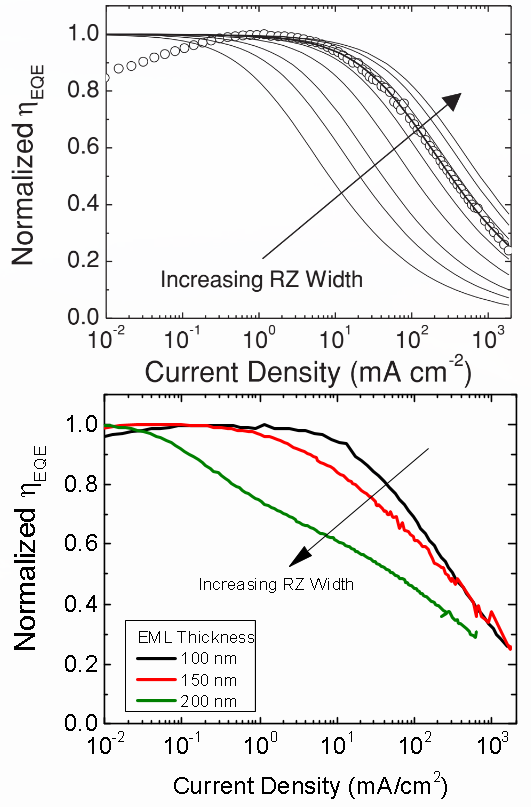
\includegraphics[width=0.48\textwidth]{unified/rz_dependence}
\caption{(a) Efficiency roll-off predicted by Erickson \textit{et al.} 2014 as a function of recombination zone width.\supercite{Erickson2014} (b) Observed efficiency roll-off for gradient EML devices.}
\label{fig:rz_dependence}
\end{wrapfigure}

In addition to the problems with the transient electroluminescence, the interpretation of the existing model without a full dynamics picture can lead to false predictions.  
Figure \ref{fig:rz_dependence}a shows what a quenching model predicts for the roll-off as a function of increasing recombination zone width.\supercite{Erickson2014}
However, even in the most idealized case of a gradient emissive layer device, where no additional interfaces come into play, the predictive model fails to replicate the behavior, as shown in Figure \ref{fig:rz_dependence}b.
While this device is of little interest for further investigation due to the extreme thickness, the point stands that this model has glaring assumptions for it's applications.

Both the transient EL and the recombination zone dependence issues arise due to an incomplete picture of the device physics, more specifically in the area of polaron dynamics.  
This work sought to address these issues by including polaron dynamics.  
Since the steady-state solution of existing models is able to accurately replicate steady-state performance, the transient EL is utilized as well as the steady-state solution to ensure that the underlying physics are accurately captured.
A valid solution should be able to accurately fit both regimes using the same model parameter values.
In order to leverage previous work, the archetypical green-emitter tris[2-phenylpyridinato-c$_2$,N]Iridium(III) (Ir(ppy)$_3$) is used for the extensively characterized photophysics.\supercite{Baldo2000,Baldo2000a,Tsuboi2006,Adachi2001a,Kawamura2006,Kawamura2005c}

%---------------------------------------------------------------------------------------------
\section{Theory}
\subsection{Exciton Dynamics}
The dominannt processes that influence the exciton population, first formalized by Reineke \textit{et al.}\supercite{Reineke2007}, have been identified as natural exciton decay, via radiative and non-radiative processes, triplet-triplet annihilation, triplet-polaron quenching, and exciton generation.\supercite{Erickson2014,Song2010}
In triplet-triplet annihilation, two triplets are able to interact, and one exciton transfers its energy to the other, resulting in one molecule relaxing to the ground state and the other forming a hot exsupercited state.
This hot state releases this additional energy to heat and typically relaxes back to the $T_1$ state.  
Triplet-polaron quenching is the interaction of a polaron with a nearby triplet exciton.
Here, one of the charges of the exciton non-radiatively recombines with the polaron of the opposite charge, leaving a remaining loose charge.
Excitons are also subject to field dissociation, but this mechanism is ignored in this work.
Field dissociation is typically observed for fields larger than $2.5 \times 10^6$ V/cm.  
This is near the maximum field used for this study, and would be important to consider for higher voltage characterization.

In agreement with previous models, singlet-triplet exciton intersystem crossing and host-guest exciton energy transfer are assumed to be fast compared to exciton decay.\supercite{Reineke2007,Baldo2000a,Turro1991a}
Since these mechanisms are much faster, they will not be rate-limiting processes and can thus be omitted from the differential equations model without sacrificing accuracy.
Within an operational device, electron and hole populations are indistinguishable.
Therefore, the electron ($n_e$) and hole ($n_h$) densities are treated as a single geralized polaron population, $n_{pol}=n_e+n_h$.
For simplicity, the model developed here treats the exciton and polaron populations as spatially uniform and confined to the exciton recombination zone.  An spatial inhomogeneity in exciton and polaron density as well as their overlap is absorbed into the bimolecular rate constants.
It is important to note that due to this assumption, rate constants are a property of the device stack, and not just a material property.
With these assumptions, the dynamic processes determining exciton density ($n_{ex}$) can be summarized in the following one-dimensional rate equation:

\begin{equation}
%\frac{dn_{ex}}{dt} = - \frac{n_{ex}}{\tau}-\frac{1}{2}k_{TT}n_{ex}^2-k_{TP}n_{pol}n_{ex}+G_{ex}
\frac{dn_{ex}}{dt} = - \frac{n_{ex}}{\tau}-\frac{1}{2}\ktt n_{ex}^2-\ktp n_{pol}n_{ex}+G_{ex}
\label{eqn:exciton_rate}
\end{equation}

where $\tau$ is the natural exciton lifetime, determined by the radiative ($k_r$) and non-radiative ($k_{nr}$) decay rates by $\tau=1/(k_r+k_{nr})$, \ktt is the rate constant for triplet-triplet annihilation, \ktp is the rate constant for triplet-polaron quenching, and $G_{ex}$ is the exciton generation rate.  
As this is a one-dimensional model, $G_{ex}$ is a spatially uniform generation rate, a simplifying assumption.
Many studies have modeled the exciton recombination zone profile, relying on material energy levels, as well as mobilities.\supercite{Rihani2006,Hassine2001,Hassine2002,Ruhstaller2003,Ruhstaller2001}
While these models are more accurate and explicit, in the way that they capture the physics, they also increase the dimensionality of our model, as well as increasing the parameterization; requiring seperate electron and hole rate equations, mobilities and energy levels for every material.
Even with this increased accuracy of the physical processes, identifying if the predicted exciton recombination zone is accurate requires significant additional measurements.
Since the goal of this work is to provide a functional model to accurately predict the transient and steady-state device behavior, spatially uniform dynamics are assumed.
Here, exciton formation is treated using a Langevin recombination formalism based on the polaron density.\supercite{Ruhstaller2003,Pinner1999,Blom1996}

\begin{equation}
G_{ex}=\frac{\kf}{4}n_{pol}^2
\label{eqn:exciton_formation}
\end{equation}

where \kf is the rate constant for exciton formation.  The factor of four accounts for the diversity of the polaron population and assumes that electrons and holes are in equal proportion.  
The accuracy of this prefactor is reduced for imbalanced charge, and is investigated in Section \ref{sec:charge_imbalance}.
For $n_e$:$n_h$ ratios 2:1 or better, less than 20\% error is found in this term.  

\section{Polaron Dynamics}

Previous models for efficiency roll-off have ignored polaron dynamics and assumed that all polarons readily form excitons.  The steady-state polaron density is then modeled using a space charge limited model.\supercite{Pope1999}
To attribute physics to this process, a simple picture of polaron dynamics is assumed, consisting of charge injection and transport, exciton formation, and polaron loss.  
In order to preserve our one-dimensionality, polarons must be uniformly distributed.  
Without competing losses in the tranport layers, all injected polarons must eventually reach the emissive layer.  
We further assume that polarons easily enter that emissive layer and that the majority of polaron build up occurs within the emissive layer, rather than the transport layers.
Therefore, the charges injected from the current density, $J$, are uniformly generated in the emissive layer by $G_{pol}=2J/ew$.  Here, $e$ is the electron charge, and the factor of two arises from an assumption of equal charge injection.  In a well balanced device, the measured current forms holes on one side of the device and electrons on the other, and are both injected into the device.  
This is discussed extensively in Section \ref{sec:carrier_injection}
Polaron losses to exciton formation mirror the exciton formation rate presented in Equation \ref{eqn:exciton_formation}, though at twice the rate due to two polarons forming one exciton.

The introduction of polaron loss from the emissive layer through the device without forming excitons is essential to address the limitations of previous models.  
Without this term, peak internal quantum efficiency of all devices is assumed to be 100\% and and the roll-up of efficiency at low current can not be explained.  
In order to capture polaron loss, a first order approximation is made for loss in that only the majority charge carrier can be lost and leaks through the device with a characteristic time, $\tau_l$.
With these mechanisms, the full polaron dynamics can be expressed as:




\begin{equation}
\frac{dn_{pol}}{dt}=\frac{-\kf}{2}n_{pol}^2-\frac{n_{pol}}{\tau_l}+G_{pol}.
\label{eqn:polaron_rate}
\end{equation}

\subsection{Transient Electroluminescence} \label{sec:transient_el}

In this work, given a full model for polaron dynamics, the model is easiest to solve starting from the application of the current pulse, rather than at peak luminace.
Under pulsed electrical excitation, Equations \ref{eqn:exciton_rate} and \ref{eqn:polaron_rate} can be solved at the beginning of the pulse with the initial conditions $n_{ex}=n_{pol}=0$.  
Upon the application of a voltage pulse, there is a time delay before polarons reach the emissive layer, as evidenced by the delay in luminance turn on.  
This has been previously attributed to charge injection and transport in the emissive layer.\supercite{Wei2004}
The injection time varies with device area due to the device capacitance and accounts for the majority of the delay time for large devices.
Transport is dependent on the mobility, as well as the field, which is a function of time due to the device capacitance.  
These times can be well predicted using the following equations:

\begin{equation}
t_{inj}=\tau\log\left(1-\frac{V_{th}}{V_0}\right)
\end{equation}

\begin{equation}
d=\int_0^{t_{trans}}\mu_0 E_0 \exp \left( \sqrt{\gamma E_0\left[1-\left(1-\frac{V_{th}}{V_0}\right)e^{-t/\tau}\right]}\right)\left[1-\left(1-\frac{V_{th}}{V_0}\right)e^{-t/\tau}\right] dt
\end{equation}

\begin{wrapfigure}{R}{0.5\textwidth}
\centering
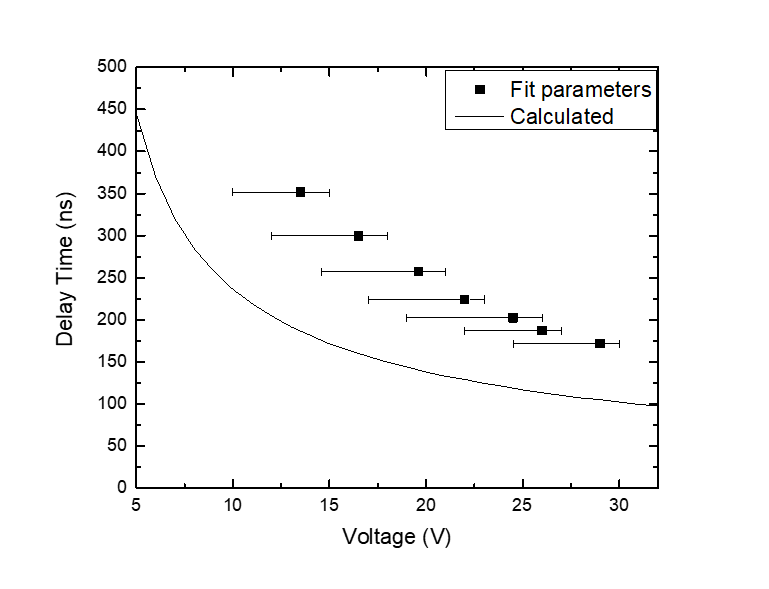
\includegraphics[width=0.48\textwidth]{unified/transport}
\caption{Extracted polaron injection time is shown as a function of voltage along with a fit from the model.}
\label{fig:transport}
\end{wrapfigure}

where $\tau$ is the RC time constant of the device, $V_{th}$ is the voltage injection threshold, $t_{inj}$ is the injection time, $t_{trans}$ is the transport time, $d$ is the tranport layer thickness, $\mu_0$ is the base mobility, $\gamma$ is the field dependent mobility term, $E_0$ is the field and $V_0$ is the voltage.
A prediction of the delay time as well as experimental values are shown in Figure \ref{fig:transport}.
Interestingly, the functional dependence of the model accurately reproduces the extracted data.
The mismatch in absolute value is due to the use of the geometric capacitance in the model, and requires a scaling factor of 2.5 of the geometric capacitance for the calculated and fit delay times to agree.  This factor is similar to that predicted by Liu \textit{et al.} for similar structures.\supercite{Liu2012d}
This suggests that the effective charge distribution in our devices is about twice as wide as the emissive layer.


After this delay, constant current polaron generation is assumed for the remainder of the voltage pulse to calculate polaron generation.  
When the voltage pulse is removed, $G_{pol}$ goes to 0 and the decay can be solved using Equations \ref{eqn:exciton_rate} and \ref{eqn:polaron_rate}.
This model does allow polarons to continue to form excitons after the voltage has been removed.
In the transient regime, if the pulse width is shorter than $\tau_l$, polarons are not able to traverse the emissive layer during the voltage pulse.  
Once the voltage is removed, there is no longer a driving force for polaron leakage via drift.
Under this assumption, the leakage term in Equation \ref{eqn:polaron_rate} can be ignored.
After the full device behavior is fit, the validity of this assumption can be assessed based on the fit values for $\tau_l$.



\subsection{Efficiency Analysis}

The maximum external quantum efficiency of an OLED is often expressed as\supercite{Baldo1998a,Rothberg1996}

\begin{equation}
\eqe=\oc \pl \chi \ef
\label{eqn:eqeSimple}
\end{equation}

where \eqe is the external quantum efficiency, \oc is the out-coupling efficiency, \pl is the photoluminescence efficiency of the emissive molecule, $chi$ is the fraction of excitons that are quantum mechanically allowed to emit (In the case of phosphorescent molecules, $\chi=1$ and $\gamma$ is  typically referred to as the charge balance.
While frequently applied, this expression suffers from two major limitations: first, there is no accounting for losses due to exciton quenching, and second, charge balance losses are not strictly defined.  
Since this equation is intended for the maximum efficiency, further modification would have to be done to account for quenching, as is done in Chapter \ref{sec:integrated_lifetime}.
The charge balance factor, $\gamma$ is typically used as a correction factor to account for differences between the observed \eqe and the other calculated factors in Equation \ref{eqn:eqeSimple}.
It is widely hinted at that charge balance relates to the carrier balance, but no formalism is ever given, so it cannot be calculated.
Given our full dynamics model, we are able to be explicit in both of these areas in a meaningful way.  
The internal quantum efficiency of a device is simply the ratio of the radiative exciton rate to the rate of electron injection, and we can therefore recast Equation \ref{eqn:eqeSimple} as


\begin{equation}
\eqe=\oc \frac{n_{ex}k_r}{G_{pol}/2}.
\label{eqn:eqeReform}
\end{equation}

Note that in this equation, exciton quenching is accounted for in the $n_{ex}$ term because in the steady-state, $n_{ex}$ is reduced according to this quenching, which is competative with $k_r$.
Dynamically, the charge balance factor is the fraction of injected polarons contributing in exciton formation.  
This can be viewed as the efficiency of Equation \ref{eqn:polaron_rate} to form excitons.
Given this interpretation, we will recast the charge balance factor $\gamma$, as an explisupercitely defined exciton formation efficiency \ef as

\begin{equation}
\ef=\gamma = \frac{\frac{1}{2}\kf n_{pol}}{G_{pol}}=\frac{\frac{1}{2}\kf n_{pol}}{\frac{1}{2}\kf n_{pol}+\frac{1}{\tau_l}}
\label{eqn:exciton_formation_polarons}
\end{equation}

Equations \ref{eqn:eqeReform} and \ref{eqn:exciton_formation} allow us to rigorously tie \eqe and \ef to dynamic processes within the device in a quantitative manner.

\section{Experimental Details} \label{sec:experimental_details}

Devices used for measurements of transient and steady-state EL had the following structure: ITO (150 nm)/poly(3,4-ethylenedioxythiophene)-poly(styr- enesulfonate) (PEDOT-PSS) (40 nm)/tris(4-carbazoyl-9- ylphenyl)amine (TCTA) (30 nm)/10\% tris[2-phenylpyridi- nato-C2,N]Iridium(III) (\irppy) doped in 4,40-Bis(N- carbazolyl)–1,10-biphenyl (CBP) (10 nm)/bathophenanthro- line (Bphen) (30 nm)/LiF (1 nm)/Al (100 nm). 
Transient PL decays were measured using 60-nm-thick films of CBP doped with 10\% \irppy deposited on quartz slides. 
The hole-only device structure used for steady-state PL quenching measure- ments had the following structure: ITO (150 nm)/PEDOT-PSS (40 nm)/10\% \irppy in CBP (60 nm)/Au (50 nm). The gold cathode was used to prevent electron injection. 
Transient EL measurements were conducted using a voltage pulse generator (HP 8114a) with pulse amplitudes ranging from 5–40V and pulse widths ranging from 250 ns–500 ns with a period 500 ls. 
Luminescence was recorded using a set of collection lenses focused onto a fast photodiode (Thorlabs DET36A). 
Pulsed \eqe measurements were conducted using the HP 8114a pulse generator until the device reached steady state current and luminance, which were recorded.  
Overlapping points with the steady state \eqe measurement were used to calibrate the luminance-current ratio to the \eqe.
The photodiode signal was recorded using an oscilloscope (Tektronix TDS5104b). 
Transient PL measurements were collected using a
pulsed nitrogen laser (Optical Building Blocks) with a pulse length of approximately 1 ns and emission wavelength of $\lambda$= 337 nm at a repetition rate of 6 Hz. Laser light was focused on the sample using a series of lenses, with collec- tion carried out using the same techniques already described for transient EL. 
Incident laser power was measured using a Coherent EnergyMax 10MB-HE detector. 
Film thicknesses and optical constants used for modeling the out-coupling efficiency in Eq. (9) were obtained using a J. A. Woollam variable angle spectroscopic elllips- ometer (VASE) using a Cauchy dispersion model.



\section{Exciton Quenching in Photoluminescence}\label{sec:pl_measurements}

\begin{wrapfigure}{R}{0.5\textwidth}
\centering
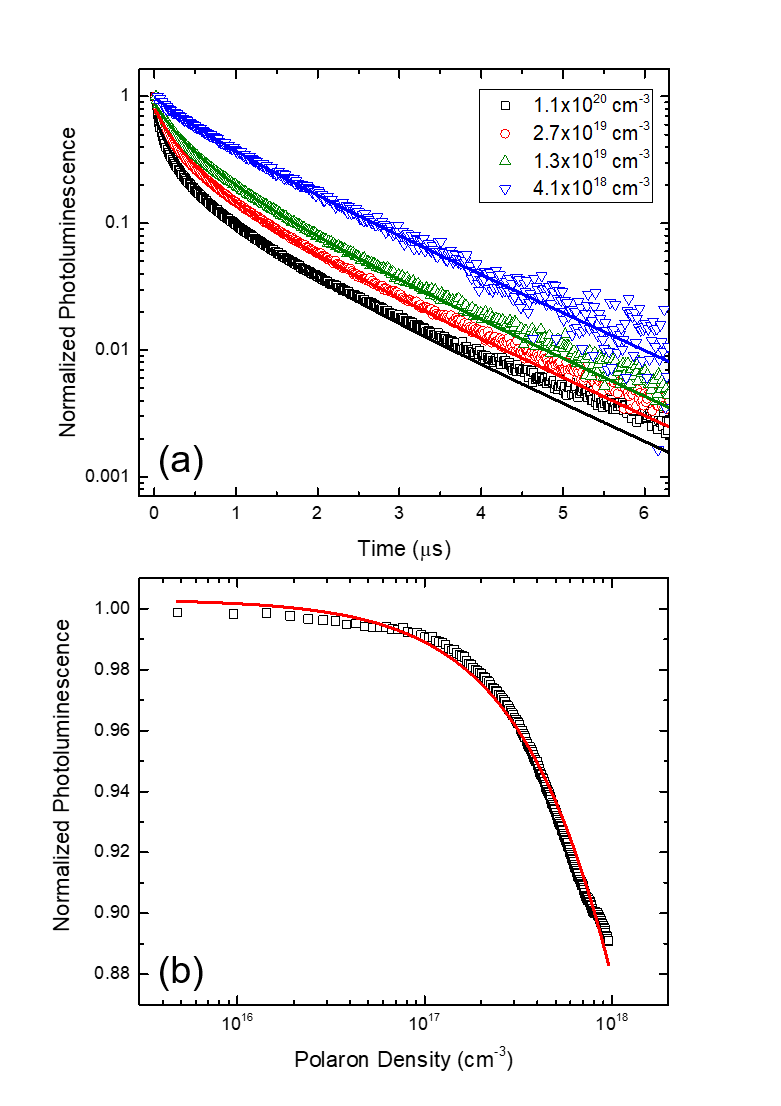
\includegraphics[width=0.48\textwidth]{unified/PL_fitting}
\caption{(a) Transient photoluminescence (PL) decays for several initial exciton densities with fits shown as solid lines using Eqn. \ref{eqn:exciton_formation}.  Fit parameters are discussed in SECTION.  Exciton densities are calculated using measured incident power and beam size in combination iwht Beer's Law.  (b) Steady-state PL quenching as a function of polaron density and the resulting fit from Eqn. \ref{eqn:ktpFit} shown as the solid line.}
\label{fig:PL_fitting}
\end{wrapfigure}

Photoluminescence measurements have been previously used to extract the rate constants for triplet-triplet annihilation and triplet-polaron quenching.\supercite{Erickson2014,Reineke2007}
This is important because it allows an independent confirmation of the extracted rate constants extracted during the electroluminescence fitting.
The transient photoluminescence exposes the natural exciton lifetime, $\tau$ and at high incident flux, the triplet-triplet annihilation rate constant, \ktt.
This measurement involves an incident laser pulse, in this case, from a 337 nm nitrogen laser, which is able to exsupercite a large exciton population.
The pulse width of the nitrogen laser is ~1ns and is much faster than $\tau$ or \ktt, allowing us to use Equation \ref{eqn:exciton_rate} with the initial boundary condition $n_{ex}=A(E_{\text{pulse}}/hfV)$ where $A$ is the absorbed fraction of photons, $E_{\text{pulse}}$ is the pulse energy, $hf$ is the photon energy and $V$ is the film volume.
Since this is optical only excitation, the other boundary condition is $n_{pol}=0$ and we can ignote Equation \ref{eqn:polaron_rate}.\supercite{Reineke2007,Erickson2014,Baldo2000a}
For CBP films doped with \irppy, good agreement with the model is observed across a range on initial exciton densities, as shown in Figure \ref{fig:PL_fitting}(a).
The exciton lifetime, $\tau$ was found to be mostly independent of exciton density and was globally fit to 1.5$\pm$0.2 $\mu s$.  
The triplet-triplet annihilation rate constant appears to be a function of intensity and ranges from $\ktt=2.4\times10^{-13}$ cm$^3$/s at $n_{ex_0}=4.1\times10^{18}$ cm$^{-3}$ to $\ktt=6.9\times10^{-14}$ cm$^3$/s at $n_{ex_0}=1.1\times10^{20}$ cm$^{-3}$.
These extracted values and trend with intensity are in good agreement with previous reports.\supercite{Reineke2007,Erickson2014,Staroske2007}
It is important to note, that the exciton environment is very important for these values.  
Previous studies have shown that the presence of a metal cathode on top of thhe film can significantly reduce the exciton lifetime by allowing additional non-radiative recombination via surface plasmon coupling.\supercite{Song2011}
This becomes important in the comparison of these parameters with those obtained under electroluminescence within a device.
A more representative experiment would have involved a full device stack with cathode, rather than just a film.  
Alas, I did not have that forsight for this experiment.



Triplet-polaron quenching rate constant measurement is done in single carrier devices as a function of polaron density.  
It is largely uninvestigated as to the differences between electrons and holes, but in previous works, hole only currents are used, a precident which will be followed in this work.\supercite{Erickson2014,Reineke2007}
A steady-state exciton population is generated optically, in this case, a 405 nm laser.  
In a single carrier device, a space charge limited current model featuring an exponential trap distribution is often used.\supercite{Lampert2002a,Giebink2009a,Pope1999}
This model is employed largely because it fits the obtained current-voltage behavior most closely.  
In reality, a single trap state would be expected, as that is what is introduced by \irppy in a doped film.  
These models are frequently employed, despite their inaccuracies, largely for simplicity.  A more accurate determination of polaron density is discussed in Chapter \ref{sec:polaron_density_measurement}.
However, in a space charge limited model with an exponential trap distribution, the current density voltage relationship can be modeled using

\begin{equation}
V=\left[ \frac{J}{e\mu N_C}d^{2l+}\left( \frac{eN_0k_BT_t}{\epsilon} \right)^l \right]^{\frac{1}{l+1}}=CJ^{\frac{1}{l+1}},
\label{eqn:ktpVoltage}
\end{equation}

where $N_C$ is the density of states at the transport level, $\epsilon$ is the permittivity, $\mu$ is the mobility, $L$ is the device thickness and $l=T_t/T$ with $T_t$ being an experimentally determined characteristic temperature of the trap distribution.  The Polarond density is then given by

\begin{equation}
n_{pol}=eN_c\left(\frac{\epsilon V}{ed^2N_0kT_t}\right)^l.
\label{eqn:kptDensity}
\end{equation}

Combining Equation \ref{eqn:kptDensity} with Equation \ref{eqn:exciton_rate}, the ratio of the steady-state PL intensity (L) to the PL intensity in the absence of polarons (L$_0$) can be written as\supercite{Reineke2007}

\begin{equation}
\frac{L(n_{pol}}{L_0}=\frac{1}{1+\tau \ktp n_{pol}}
\label{eqn:ktpFit}
\end{equation}

After fitting the current density-voltage characteristics of the device are fit using Equation \ref{eqn:ktpVoltage}, Equations \ref{eqn:kptDensity} and \ref{eqn:ktpFit} can be used to extract the triplet-polaron rate constant for a given value of $\tau$.  
In this case, we use $\tau$ as extracted from the transient PL measurements.
The fit obtained for a CBP \irppy hole only device is shown in Figure \ref{fig:PL_fitting}b.
This devices utilizes a gold cathode to prevent electron injection and shows minimal exciton formation, as expected.
The organic stack is the same as the emissive layer of the inviestigated device.  
In fitting the current density-voltage characteristics using Equation \ref{eqn:ktpVoltage}, a value of $l=(2.4\pm0.2)$ was found.  
The extracted triplet-polaron quenching rate constant from fitting Equation \ref{eqn:ktpFit} was $\ktp=(2.8\pm0.2)\times 10^{-13}$ cm$^3$/s and is agreement with previous measurements.\supercite{Erickson2014,Reineke2007}


\section{Application to Devices}

In order to fit both the steady-state and transient regimes, decisions need to be made as to a methodology for extracting parameters.  
The obvious choice may seem to be to try to produce a global fit by fitting both regimes simultaniously.  
The major draw back of this approach is the value of $\tau_l$.  
Since this is a function of the applied field, this is not single valued and relies on knowing the field dependence.
Additionally, the steady-state provides little insight into the actual quantities of $\tau$, \ktt, \ktp, and \kf, and only the ratio of radiative and non-radiative processes is needed for a quality fit of the efficiency roll-off.
Additionally, within this model, only $n_{ex}$ is experimentally available to fit, and the fit parameters are not independent.
The most obvious example of this is the values of \ktt and \ktp, which have similar impact on the exciton population and similar formulation.  
This makes it near impossible to distinguish a dominant mechanism between these two, and results for exact values of quenching constants need to be considered with caution.
This methodology only gives a net effect of the two quenching mechanisms in total, rather than a true seperate measurement of both quantities as is obtained in the PL quenching measurements, discussed in Section \ref{sec:pl_measurements}.

With these limitations addressed, the method used for this discussion to fit all of the device physics has been carefully considered to achieve the highest parameter sensitivity.
The bimolecular quenching constants are most sensitive to the efficiency roll-off since small changes in the quenching constants make a large impact on the roll-off behavior.
However, the lifetime and exciton formation can only be determined to within a fixed ratio.
In contrast, the exact values of lifetime and exciton formation rate are critical to the behavior of the transient EL while the bimolecular quenching constants are difficult to probe in the current regime investigated.
In order to use these sensitivities, a quenching only model (ignoring $\tau_l$) to fit the normalized efficiency roll-off, such has been previously reported, is used to determine the bimolecular quenching rates, \ktt and \ktp.  
Quenching only models can only fit the normalized \eqe roll-off because without a polaron loss term, \ef is assumed to be 100\% and the exact magnitude of efficiency cannot be reproduced.
Initial values for all parameters, except \kf which is previously unmeasured, are determined by the photoluminescence measurement values.
With these quenching rates fixed, the transient EL is fit using Equations \ref{eqn:exciton_rate} and \ref{eqn:polaron_rate} in order to determine $\tau$ and \kf.
Remember that in the transient regime for short pulses, we can assume that $\tau_l=\infty$ and can be ignored.

With these critical rate constants determined, we will revisit the efficiency as a function of current density.
In the first pass, we ignored the exact value of efficiency and only fit the normalized roll-off.
Now, since we know the other parameters, we can revisit \eqe, now matching the exact profile for all currents, by conducting a point-by-point fit for $k_F$.
This fit for $k_F$ can then be used to calculate \ef and can be compared to a drift model, to assess its validity.


\subsection{Quenching Only Steady-State Fit}\label{sec:eqe_fitting}

\begin{wrapfigure}{R}{0.5\textwidth}
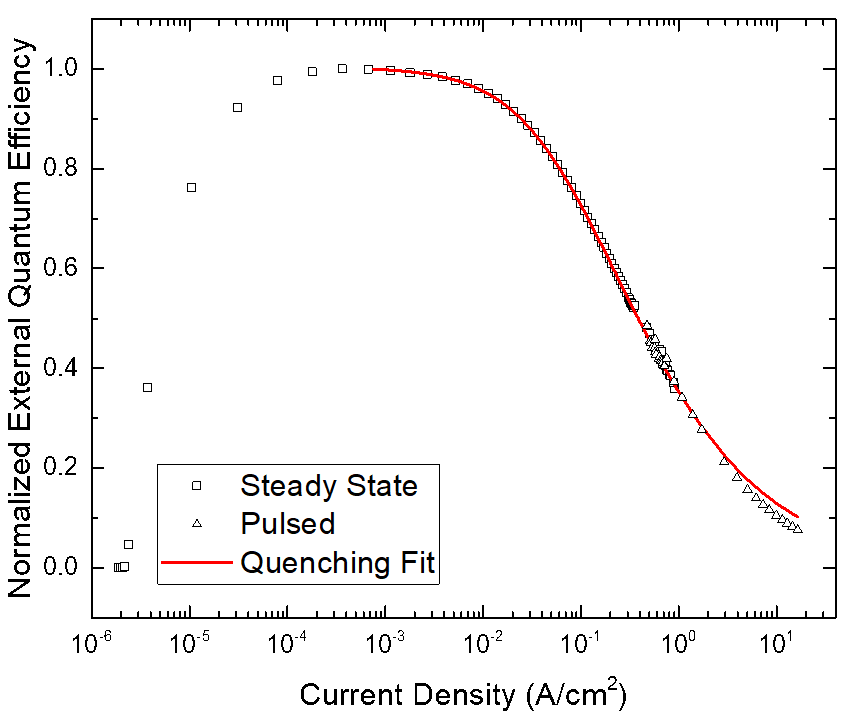
\includegraphics[width=0.48\textwidth]{unified/rollOffFit}
\caption{Normalized experimental \eqe as a function of current density.  Solid line is a fit to the data using Eqn. \ref{eqn:exciton_rate} and \ref{eqn:polaron_rate} in the absence of polaron loss.  Pulsed eqe measurements are conducted using low duty cycle pulses to steady-state luminance to reduce Joule heating in device.}
\label{fig:rollOffFit}
\end{wrapfigure}

To measure transient and steady-state EL, devices were constructed using the architecture discussed in Section \ref{sec:experimental_details}.  
These devices had an \eqe of $(9.7\pm0.1)$\%.  Equations \ref{eqn:exciton_rate} and \ref{eqn:polaron_rate} were used to fit the peak normalized steady-state efficiency roll-off with $\tau_l=\infty$.  Again, omitting a polaron loss term, this model assumes that all roll-off behavior comes from quenching.  
Parameters were initialized using the values obtained from PL quenching measurements, described in Section \ref{sec:pl_measurements}.
An experimental fit is shown in Figure \ref{fig:rollOffFit} and shows good agreement, except at very high currents associated with pulsed \eqe measurements.  
Parameters are summarized in Table \ref{tab:fit_parameters} and are in good agreement with those previously reported.\supercite{Reineke2007,Baldo2000a}



\begin{table}[h]
\centering
\begin{tabular}{c|c|c}
& Transient EL & Efficiency Roll-off \\
\hline
$\tau$ (s) & $6.9\pm 0.1 \times 10^{-7}$ & $6.1 \times 10^{-7}$ \\
\ktt (cm$^3$/s) & $7.1\times 10^{-12}$ &$7.1\times 10^{-12}$ \\
\ktp (cm$^3$/s) & $3.3\times 10^{-13}$ &$3.3\times 10^{-13}$ \\
\kf (cm$^3$/s) & $7.7\pm3.5\times 10^{-12}$ &$1.6\times 10^{-11}$ \\
\end{tabular}
\caption{Fit parameters extracted from transient and steady-state electroluminescence.  Transient EL fit parameters averaged over all measured current densities.  \eqe roll-off parameters averaged over several measured devices.  Triplet-triplet annihilation and triplet-polaron quenching rates are fixed to those obtained from fitting the normalized efficiency roll-off.}
\label{tab:fit_parameters}
\end{table}



\subsection{Transient Modeling}

Transient EL measurements were conducted on the same devices used for the efficiency measurements described in Section \ref{sec:eqe_fitting}. 
Pulse widths ranging between 250–500 ns with a period of 500 ls were used with current densities ranging between 0.5–50 A/cm$^2$. 
Fast Fourier Transform (FFT) filtering is used to remove experimental noise from the measured signal to increase fit accuracy. 
The bimolecular quenching rate constants are fixed to the values determined from the fitting of the steady-state efficiency roll-off (Table \ref{tab:fit_parameters}).
The exciton lifetime and exciton formation rate constant are allowed to vary to fit the transient EL and are summarized in Table \ref{tab:fit_parameters}.
The value of $\tau$ is shorter than that obtained under transient PL, likely due to the cathode present for EL trnsient studies.\supercite{Song2011}
Fits using this model are shown in Figure \ref{fig:transientFits} and show excellent agreement above the detection limit.  The initial turn on is well replicated by the luminance delay model discussed in Section \ref{sec:transient_el}


\begin{figure}[ht]
\centering
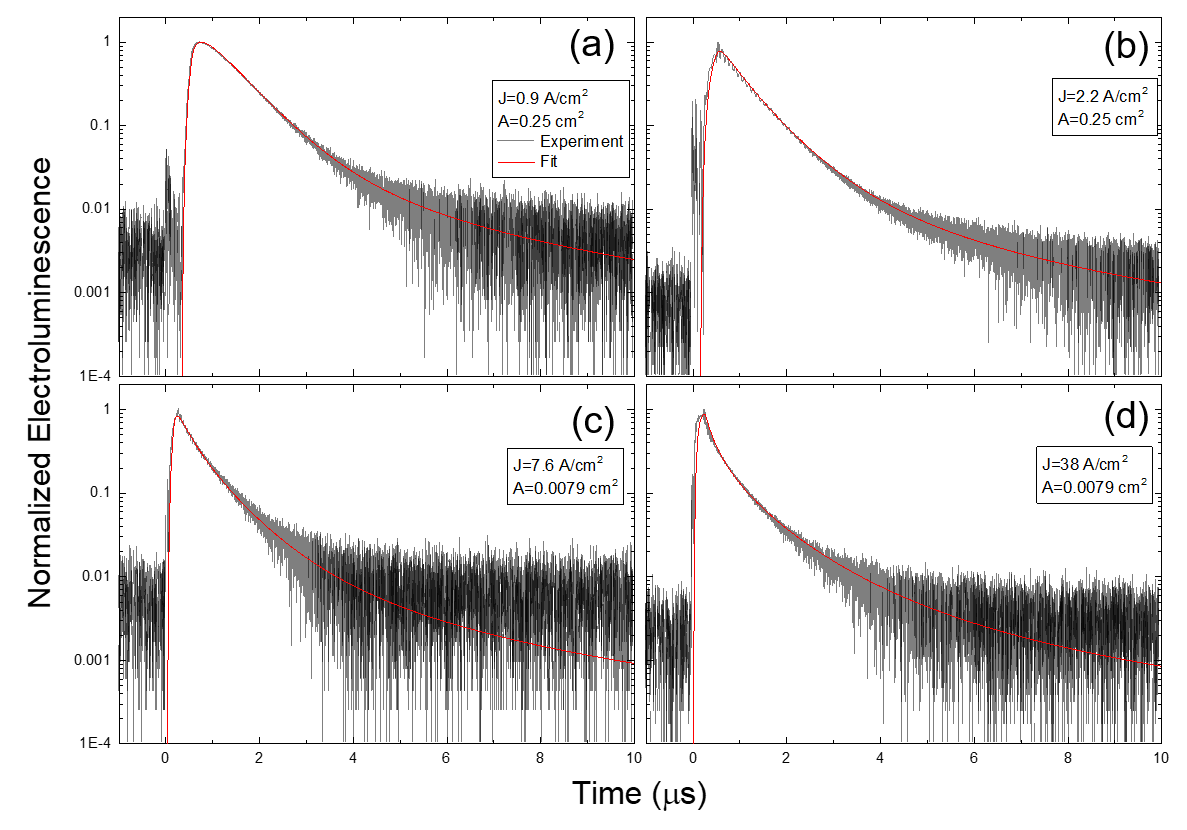
\includegraphics[width=0.8\textwidth]{unified/transientFits}
\caption{Transient electroluminescence (EL) for four different current densities (J) and device areas (A). (a) 0.25 $cm^2$ device at a current density during the pulse of J = 0.9 $A/cm^2$ (b) 0.25 cm2
device at J = 2.2 $A/cm^2$ (c) 0.0079 $cm^2$ device at J = 7.6 $A/cm^2$ (d) 0.0079 $cm^2$ device at J = 38 $A/cm^2$}
\label{fig:transientFits}
\end{figure}


\subsection{Transient Term Efficiency}

Utilizing the understanding of dynamics developed here, the efficiency of each component in Equation \ref{eqn:exciton_rate} for the transient EL can be analyzed.   
This is shown for representative high and low current density behavior in Figure \ref{fig:termEfficiency}. 
At the application of the voltage pulse, exciton generation is the dominating feature, resulting in a steep rise in luminescence. 
As the exciton and polaron populations peak, the resulting dependence is seen on the bimolecular quenching terms, leading to the curvature seen before and after the removal of the injected current. 
During the decay, the exciton and polaron populations rapidly decrease due to quenching, resulting in the natural exciton lifetime becoming the dominant behavior. 
As the exciton population further diminishes, formation of excitons from the residual polaron population is observed, resulting in the slow decay seen at long times. 
Figure \ref{fig:termEfficiency}a shows the decoupled EL transient behavior at a low current density where exciton formation and the natural lifetime are always competitive processes, resulting in the slow rollover in the experimental behavior of Figure \ref{fig:transientFits}a. 
Slightly higher current densities do not show the bimolecular terms rise to prominence, resulting in the linear decay after the pulse seen in Figure \ref{fig:transientFits}b. 
Bimolecular quenching terms show increasing importance with current density, especially at times soon after the removal of voltage. 
We see this behavior in Figures \ref{fig:transientFits}c and \ref{fig:transientFits}d with the decoupled high current density behavior of Figure \ref{fig:transientFits}d demonstrated in Figure \ref{fig:termEfficiency}. 
Here, we are able to see that bimolecular quenching events dominate when the exciton density is peaked after the removal of voltage. 

\begin{wrapfigure}{R}{0.5\textwidth}
\centering
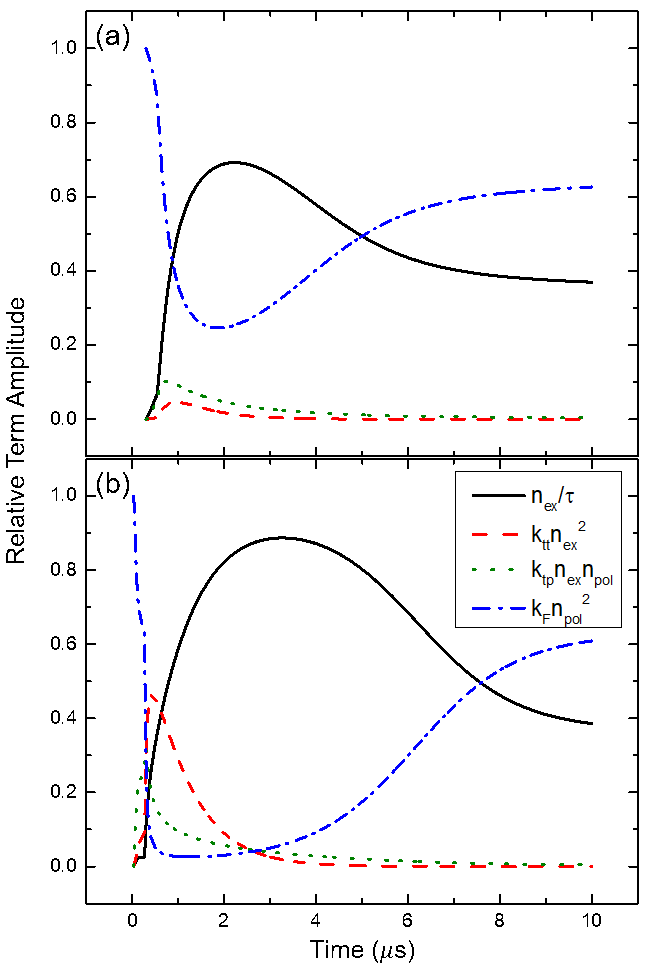
\includegraphics[width=0.48\textwidth]{unified/termEfficiency}
\caption{Term efficiency for each dynamical process influencing the exciton population for (a) 0.25 $cm^2$ device operated at 0.9 $A/cm^2$ for 500 ns and (b) 0.785 $mm^2$ device operated at a current density of 38 $A/cm^2$ for 250 ns. Relative term amplitude is calculated as the magnitude of each term in Eqn. \ref{eqn:exciton_rate} divided by the sum of absolute values of each term.}
\label{fig:termEfficiency}
\end{wrapfigure}



\subsection{Extracting Exciton Formation Efficiency}

Thus far in the fitting, the introduced model has successfully fit the transient EL and steady-state efficiency roll-off using Equations \ref{eqn:exciton_rate},\ref{eqn:exciton_formation}, and \ref{eqn:polaron_rate} by including polaron dynamics in the absence of charge leakage.
However, only the efficiency roll-off and the normalized reduction in magnitude have been modeled. 
By including the polaron transit time in the analysis, the exact magnitude can be fit for both the rise and fall of efficiency. 
Starting with the experimental \eqe as a function of current density, Equation \ref{eqn:eqeReform} can be used to find the exciton density, $n_{ex}$, as a function of current density, which in turn allows Equations \ref{eqn:exciton_rate} and \ref{eqn:polaron_rate} to be solved in the steady-state for $\tau_l$.  
The out-coupling efficiency, \oc, is separately determined using optical modeling and found to be $\oc=17.7\%$.\supercite{Furno2010,Furno2012}  
The details of this calculation are discussed in Chapter \ref{sec:out_coupling}.
The radiative rate in Equation \ref{eqn:eqeReform} can be extracted from measurements of $\tau$ and \pl as $\pl=\tau k_r$.  Once the exciton population is known, Equation \ref{eqn:exciton_rate} can be solved for the polaron population, $n_{pol}$ using the fit values from the transient EL.  With $n_{pol}$ and $G_{pol}$ known, Equation \ref{eqn:polaron_rate} can be used to extract the $\tau_l$ needed to reproduce the experimental \eqe.  
This technique produces an exact match of the shape and magnitude of the efficiency, including both the roll-up and roll-off.
This is the first time in literature that a quantitative physical explanation has been attributed to the roll-up.
Any error in this method are absorbed into $\tau_l$.
Extracted values of $\tau_l$ are shown in Figure \ref{fig:chargeBalance}.
In order to justify these values, a simple drift model explanation can be used, quantified by

\begin{equation}
\tau_l=\frac{w}{E\mu(E)}.
\label{eqn:drift}
\end{equation}

Where $\mu$ is the mobility, obtained from Parshin \textit{et al.},\supercite{Parshin2006} $w$ is the device width, and $E$ is the electric field.  
This simple explanation for $\tau_l$ holds very well at low current density, corresponding to the efficiency roll-up, as well as the peak efficiency.  
Deviation from this model occurs as current density increases past $10^{-1}$ A/cm$^2$.  
However, in this regime, exciton and charge densities are becoming increasingly high, and the predicted values become increasingly non-phyiscal.
It is expected that in this regime, this simple model described in Equation \ref{eqn:drift}, would break down.


\begin{wrapfigure}{R}{0.5\textwidth}
\centering
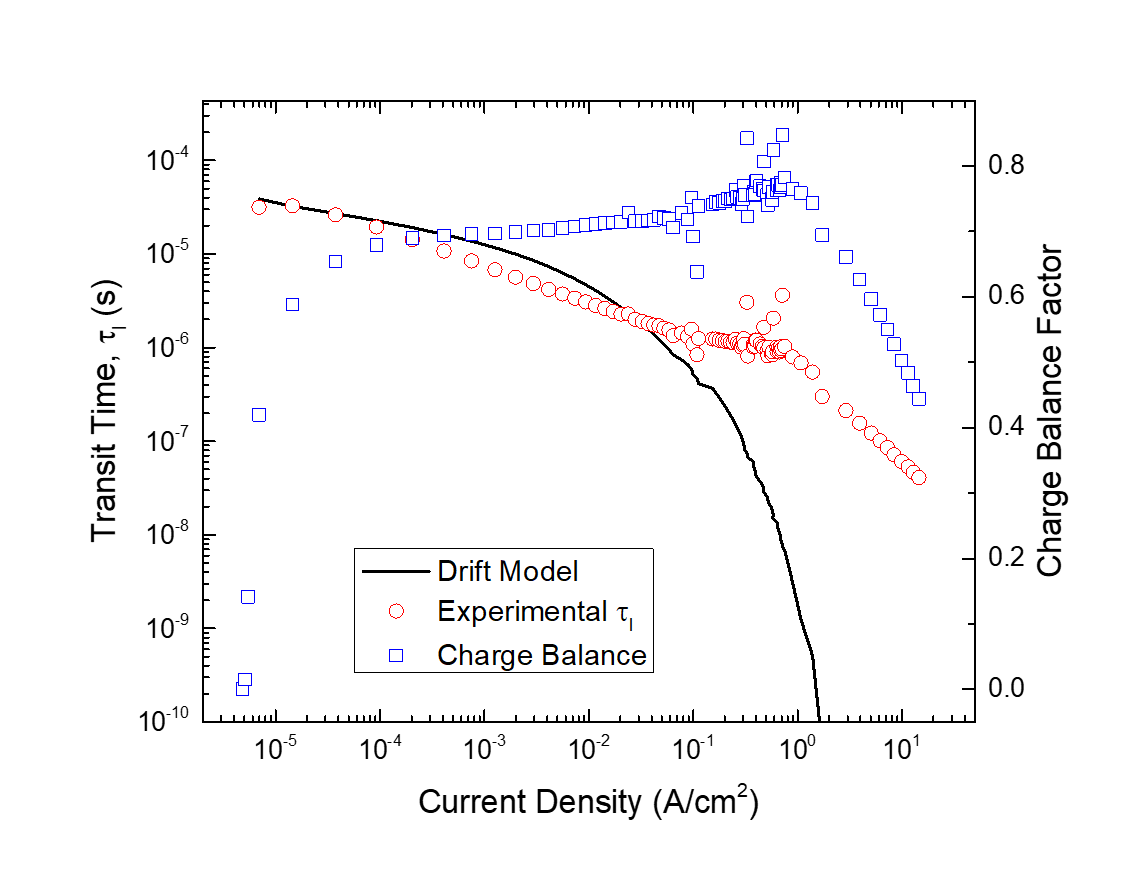
\includegraphics[width=0.48\textwidth]{unified/chargeBalance}
\caption{Transit time extracted from \eqe measurements are shown as the red circles. Predictions using the drift model are calculated using Eqn. \ref{eqn:drift}. The drift model assumes a uniform electric field. Good agreement between the experimental transit time and the drift model is found for a field distributed over 20 nm. The charge balance factor is shown as a function of current density in blue squares.}
\label{fig:chargeBalance}
\end{wrapfigure}
\subsection{Drift Model}


With the transit time known, Equation \ref{eqn:exciton_formation_polarons} can be used to find \ef, shown in Figure \ref{fig:chargeBalance}.
Charge balance remains relatively constant throughout the onset of roll-off and only falls when the efficiency approaches one quarter of its initial value. 
Using a different modeling approach, Giebink and Forrest\supercite{Giebink2008c} find that for a similar system, a larger portion of the roll-off is due to a loss of charge balance, likely due to a thicker emissive layer and differing transport layers than those used in this study. 
With the dependence of the charge balance factor on current density established, the validity of the assumption of uniform charge balance during the fit of the normalized efficiency roll-off in Section \ref{sec:eqe_fitting} can now be assessed. 
The charge balance, seen in Figure \ref{fig:chargeBalance}, remains almost constant for the majority of the roll-off but deviates at high current density, suggesting that the high current density regime should not be fit with the quenching only model. 
However, the fit shown in Figure \ref{fig:rollOffFit} is not limited by this restriction as there is excellent agreement between the model and experiment in the regime of near constant charge balance, with the only discrepancy in the fit coming at high current density where the model assumptions break down. 
Returning to fit the normalized efficiency in the regime of near constant charge balance, as defined by Figure \ref{fig:chargeBalance}, while holding $\tau$ and $k_F$ constant, \ktt and \ktp are found to be $(4.5\pm0.4) \times 10^{-12}$ cm$^3$/s and $(2\pm3)\times 10^{-12}$ cm$^3$/s, respectively.
This small variation of quenching parameters does not change the fit quality for the regime in question. 
Repeating the fitting process in this regime yields no significant differences in $\tau$ and $k_F$ or the dependence of charge balance on current density.


\section{Understanding Assumptions of Polaron Model}


In the model described in this work, electrons and holes are summarized into a generalized
polaron population with the dynamics described using Equation \ref{eqn:polaron_rate}. 
To understand the impacts that this has on calculating the polaron injection rate and the exciton formation rate, the electrons and holes must be independently examined. 
The most complete dynamics picture related to the developed model would express individual electron and hole injection as well as individual transit times. This full picture can be written as:

\begin{equation}
\frac{dn_h}{dt}=-\kf n_en_h-\frac{n_h}{\tau_{lh}}+\frac{J_h}{ew}
\label{eqn:hole_rate}
\end{equation}

\begin{equation}
\frac{dn_e}{dt}=-\kf n_en_h-\frac{n_e}{\tau_{le}}+\frac{J_e}{ew}
\label{eqn:electron_rate}
\end{equation}


where and are the electron and hole population densities, $n_e$ and $n_h$ are the electron and hole
transit times, respectively, $J_h$ and $J_e$ and are the single carrier injected currents. While more
accurate, Equation \ref{eqn:hole_rate} and \ref{eqn:electron_rate} pose several problems for replicating device behavior due to the inability to distinguish between carriers during device operation. 
This is further complicated by the inability to separately measure the single carrier injected currents and leak rates due to transit times. 
To better understand the approximations used in Eqn. (3), a detailed analysis of current injection is presented, followed by error analysis of the exciton formation term based on the composition of the polaron population.

\subsection{Carrier Injection} \label{sec:carrier_injection}


Let $J$ be the total current within our device.  
This must be maintained throughout our circuit assuming no charge buildup. 
Within the device, the total current can be written as $J=J_e+J_h$.  
Experimentally, $J$ is the only measurable current as we are not able to distinguish between electron and hole or leaked currents.  
The current incident on either contact will be referred to as  $J_1$ and $J_2$. 
These currents are summarized in Figure \ref{fig:currentDiagram}.
In the case of no leakage current, there must be complete recombination in the emissive layer.  
Therefore all of the externally measured current from one side of the device contributes only to electron current and all current on the other side contributes only to hole current.

\begin{equation}
J_1\rightarrow J_h = J_2 \rightarrow J_e
\label{eqn:current_no_leakage}
\end{equation}

This maintains constant current throughout the external circuit. 
No charges are allowed to leave the emissive layer without recombining with the opposite charge species and constant current maintains that $J_e=J_h$.  
The injected polaron density is then:


\begin{equation}
\frac{J_e}{ew}+\frac{J_h}{ew}=\frac{J_1+J_2}{ew}=\frac{2J}{ew}
\label{eqn:injected_polarons_no_leakage}
\end{equation}

\begin{wrapfigure}[15]{R}{0.5\textwidth}
%\centering
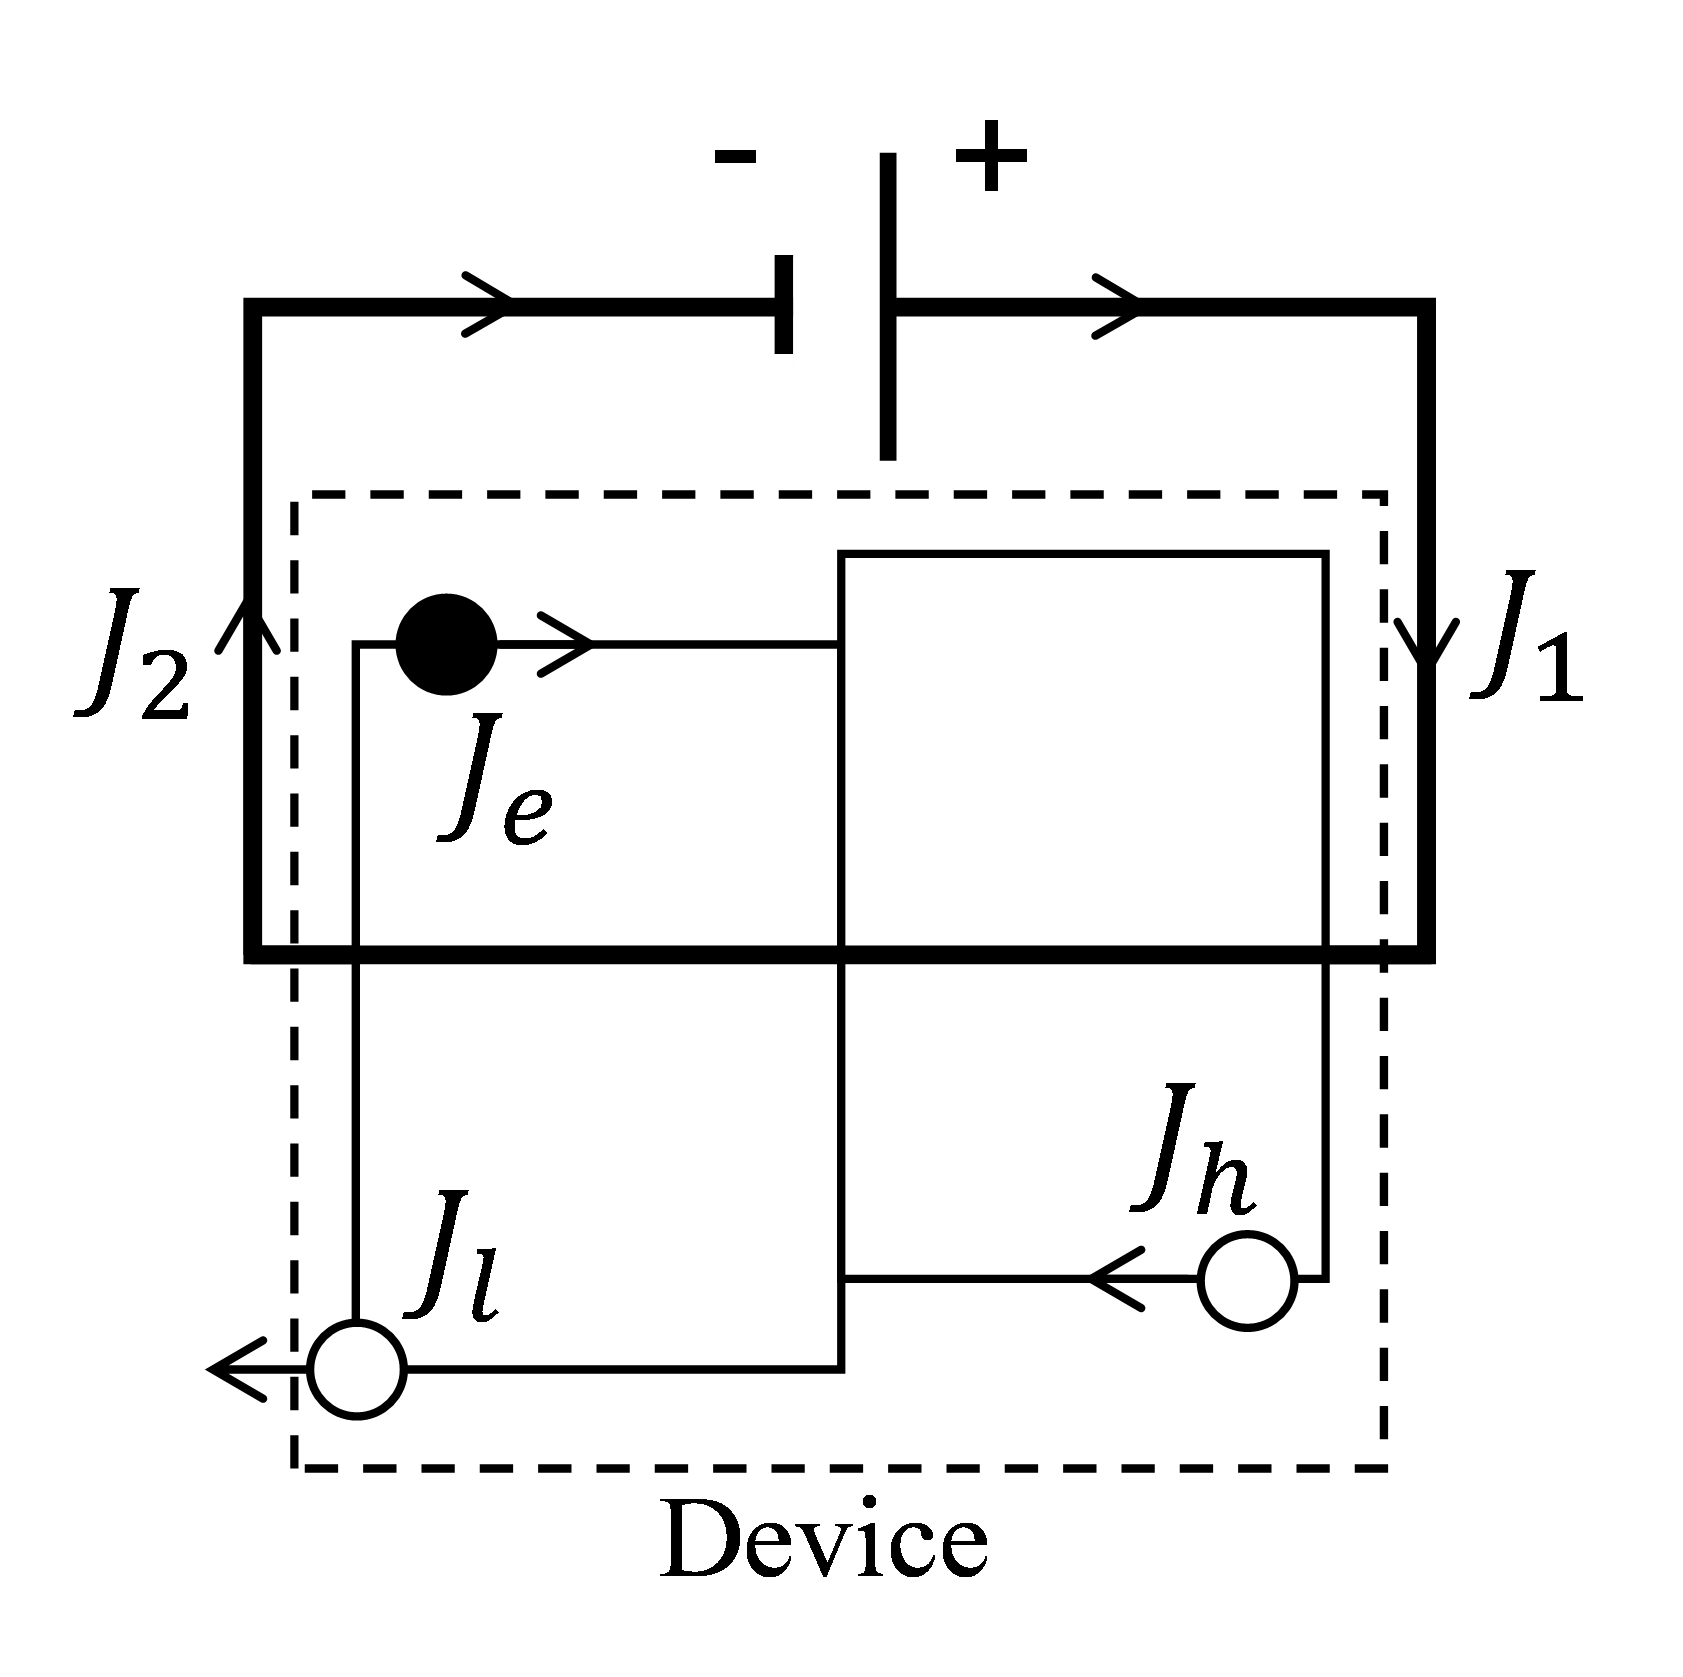
\includegraphics[width=.48\textwidth]{unified/currentDiagram}
\caption{Current density formalism within the circuit. $J_1$ and $J_2$ are the currents measured on either side of the device. $J_e$ and $J_h$ are the electron and hole currents within the device and $J_l$ is the unbalanced current, assumed to be only holes, that leaks out of the opposing contact.}
\label{fig:currentDiagram}
\end{wrapfigure}
This expression becomes more complicated when charge leakage is allowed. Let us assume that holes are the only leaking species. 
Let $J_l$ be the current leaking through the emissive layer. 
On the hole side of the device, all current is hole current. 
However, on the electron side of the device, the measured current is a combination of the electrons injected and the leaked holes.

\begin{equation}
J_1=J_h
\label{eqn:current_holes_leakage}
\end{equation}

\begin{equation}
J_2=J_e+J_l
\label{eqn:current_electrons_leakage}
\end{equation}

For current continuity, the current on either side of the device must be equal.

\begin{equation}
J=J_h=J_e+J_l
\label{eqn:current_continuity_leakage}
\end{equation}

From this expression and the experimentally measured current, it is not possible to know the electron and hole currents independently without making some assumption about the leaked current.  
If both carriers are allowed to leak, there is a leakage term on the hole current side of Equation \ref{eqn:current_electrons_leakage} as well.  
Without additional information about the proportion or magnitude of the leaked current, there is no exact expression for polaron injection in terms of $J$.  
Therefore, the approximation is used that the polaron injection and loss due to leakage can be written as:

\begin{equation}
G_{pol}-\frac{J_l}{ew}=\frac{2J-J_l}{ew}
\label{polaron_generation}
\end{equation}

This is the expression used in the final model, assuming the charge leakage can be written in terms of the total population and a transit time for leakage as  $J_l/ew=n_{pol}/\tau_l$ and $G_{pol}=2J/ew$.  
The approximation in Equation \ref{eqn:current_continuity_leakage} is strong assuming  is small relative to  $J_h$ and $J_e$.

\subsection{Charge Imbalance} \label{sec:charge_imbalance}

\begin{wrapfigure}{R}{0.5\textwidth}
\centering
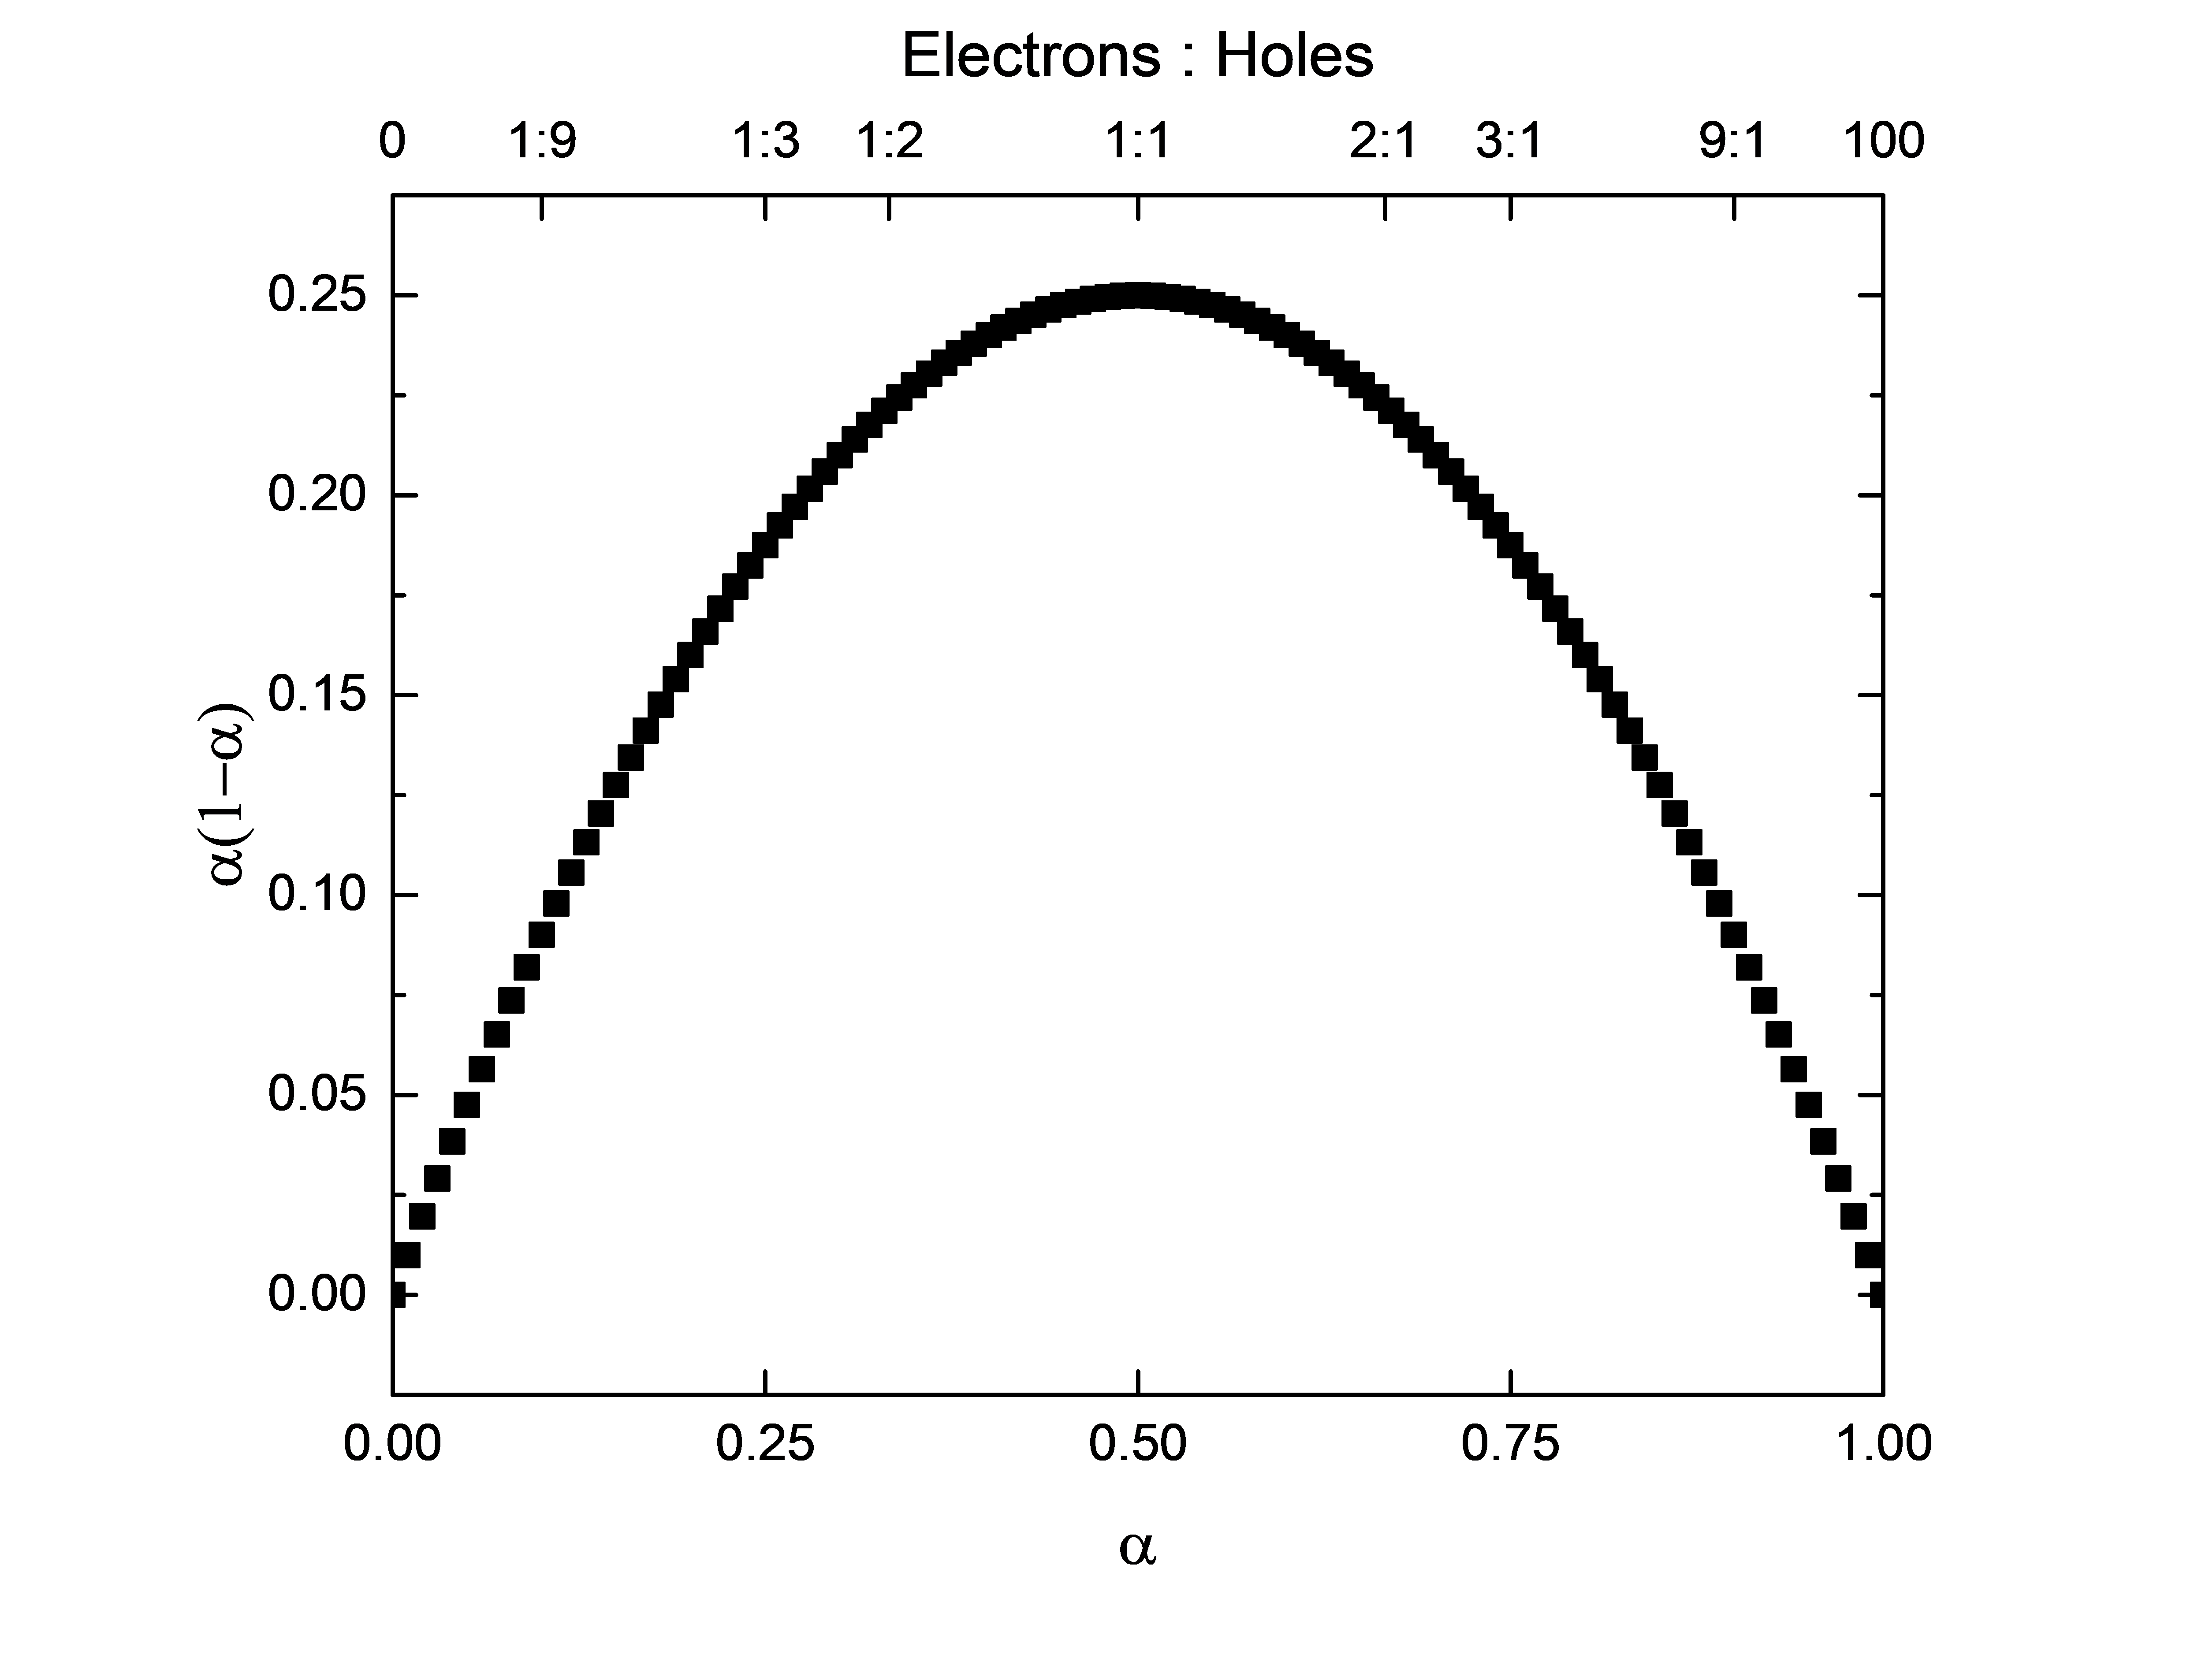
\includegraphics[width=.48\textwidth]{unified/EHratio}
\caption{The quantity $\alpha(1-\alpha)$ is plotted as a function of the polaron composition, $\alpha$ and the electron to hole ratio.}
\label{fig:EHratio}
\end{wrapfigure}

In the exciton formation term of Equation \ref{eqn:polaron_rate}, the factor of two in the denominator assumes that charges are in equal proportion.  
More generally, Equations \ref{eqn:electron_rate} and \ref{eqn:hole_rate} can be used to evaluate the error in this term as the charge balance increases.  
Let the carrier ratio be defined as:

\begin{equation}
\alpha=\frac{n_h}{n_e+n_h}
\label{eqn:charge_ratio}
\end{equation}

This is different from the charge balance we have defined in the text as this is an actual ratio of carriers, rather than the exciton formation efficiency.  
Additionally, let  $n+{pol}=n_e+n_h$ be the polaron population density.  
With these definitions, the terms for polaron loss to exciton formation of Equations \ref{eqn:electron_rate} and \ref{eqn:hole_rate} can be summed as:

\begin{equation}
\left[\frac{dn_{pol}}{dt}\right]_{formation}=-2\kf n_{pol}^2\alpha(1-\alpha)
\label{eqn:exciton_formation_charge_ratio}
\end{equation}

In the case of perfect balance, the expression  $\alpha(1-\alpha)=1/4$ and agrees with Equation \ref{eqn:polaron_rate}.  
The variation in $\alpha(1-\alpha)$ as a function of $\alpha$  can be seen in Figure \ref{fig:EHratio}.  
With charge ratios up to 1:3, there is less than a 20\% error in this expression.  
The high efficiency devices examined in this work are expected to operate in this regime, and the value of  $\alpha(1-\alpha$ should not change the value of  $k_F$ significantly.





\section{Conclusion}

A universal dynamics model has been successfully implemented that allows the fitting of the transient and steady-state EL behavior of OLEDs using \irppy as an emitter. 
This model relies upon the previously studied parameters $\tau$, \ktt, and \ktp as well as introducing polaron dynamics in the form of an exciton formation rate, $k_F$ and polaron leakage time $\tau_l$. 
This model has been used to deconstruct all features of the transient EL over three decades of decay. The fit parameters $\tau$, \ktt, and \ktp have all been verified independently using PL studies in agreement with the proposed model. 
The steady-state efficiency has been fully characterized using quenching and charge leakage through the device. 
The behavior of the investigated devices suggests that charge leakage through the emissive layer dominates the roll-up in efficiency, while bimolecular quenching is respon- sible for the majority of the roll-off in efficiency.

This model has successfully been able to model all of the device physics present in the electroluminescence behavior.  However, one of the initial goals of this project was to be able to quantify the bimolecular rate constants more effectively within a device.  In this regard, the model is not useful as \ktt and \ktp are codependent and their relative values are still unknown.  

%\ifcsdef{mainfile}{}{\bibliography{../library}}
\ifcsdef{mainfile}{}{\printbibliography}
\end{document}

